\documentclass[simplex.tex]{subfiles}
% DO NOT INCLUDE PREAMBLES/PACKAGES HERE!!
% packages are inherited from preamble.tex; you can compile this on its own
\begin{document}
\subsection[ndviz]{ndviz}

NeuroDataViz was rewritten to replace Leaflet entirely with Neuroglancer, an open-source web-based visualization tool from Google. Neuroglancer handles requesting data from a remote server and rendering data using WebGL. Whereas Leaflet requested 2D image tiles, Neuroglancer requests 3D image volumes. Although this results in a slight increase in request size, requesting 3D volumes allows Neuroglancer to render three canonical plane views (i.e. xy, xz, and yz) without requesting the data in triplicate as well as reducing latency when traveling in the z-direction. By replacing Leaflet with Neuroglancer we can add the same benefits to NDViz essentially ``for free''. 

Our first major addition to the Neuroglancer code base involved refactoring the ?SliceView? functionality to support arbitrary data types. Neuroglancer manages data loading using functionality called ?SliceView?. Tiles are requested based on the viewport and chosen plane(s) (e.g. xy). Because 3D volumes can substantially increase the data size, both data loading and data unloading become equally important. The infrastructure in SliceView manages this entire process. However, SliceView was designed solely for image data. In conjunction with Jeremy Maitin-Shepard, who developed Neuroglancer, we refactored the SliceView code to support arbitrary data formats. We then added infrastructure to manage volumes containing not image data, but point data to create ?vector graphics? layers that can display points, lines, or polylines. We are using this point layer functionality to display vector fields derived from the feature point matches between image slices (see figure).

We are planning on contributed the SliceView modifications back to Neuroglancer to share with the neuroscience community at large and are currently in the process of finalizing and integrating those changes into the main Neuroglancer repository.

%%%   EXAMPLE FIGURE BLOCK
\begin{figure}[!h]
\begin{cframed}
\centering
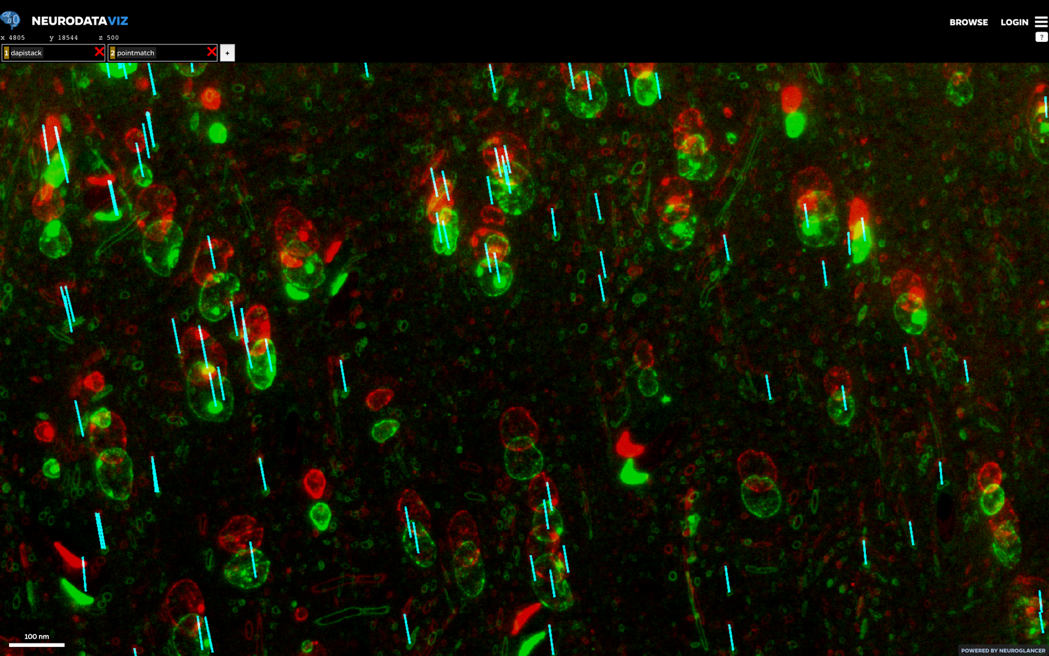
\includegraphics[width=0.95\textwidth, height = 2.75in]{../../figs/ndvizpointmatch.png}
\caption{NeuroDataViz, powered by Neuroglancer with point matches rendered as 3D lines (in cyan) overlayed on two serial sections of Array Tomography data. Data collected by Forrest Collman et al at the Allen Insitute for Brain Science, Seattle WA.}
\label{fig:name}
\end{cframed}
\end{figure}

\clearpage
\end{document}
